\section{Theory}
\begin{frame}
    \frametitle{Retarded cumulant}
\begin{align}
    A_{pq}(\omega )=-\frac{1}{\pi}G^R(\omega)
\end{align}
with
\begin{align}
G_{ii}^R(t)=-i\theta(t)\, e^{-i \epsilon_i^{\text{eff}} t} e^{C_{ii}^R(t)}.
\end{align}\pause
Using $\beta_{ii}(\omega) = \left|\operatorname{Im} \Sigma_{ii}^R\left(\omega+\epsilon_i^{\text{MF}}\right)\right|$
\begin{align}
    C_{ii}^R(t)&=\int d \omega \frac{\beta_{ii}(\omega)}{\omega^2}\left(e^{-i \omega t}+i \omega t-1\right)\\
&= \sum_{j\nu} \zeta_{ij\nu} \left[ e^{-i\Delta_{ij\nu} t} - 1 + i\Delta_{ij\nu} t \right] + \sum_{a\nu} \zeta_{ia\nu} \left[ e^{-i\Delta_{ia\nu} t} - 1 + i\Delta_{ia\nu} t \right]
\label{eq:Cpp_2}
\end{align}
with $\Delta_{ij\nu} = \epsilon_i^{\text{MF}} - \epsilon_j^{\text{MF}} + \Omega_\nu - i\eta$ and $\Delta_{ia\nu} = \epsilon_i^{\text{MF}} - \epsilon_a^{\text{MF}} - \Omega_\nu - i\eta$ with coupling weights $\zeta_{ij\nu} = \left(\frac{M_{ij\nu}}{\Delta_{ij\nu}}\right)^2$ and $\zeta_{ia\nu} = \left(\frac{M_{ia\nu}}{\Delta_{ia\nu}}\right)^2$.
\end{frame}
\begin{frame}
    \frametitle{Time-ordered cumulant}
\begin{align}
A_{p q}(\omega) & =\frac{\mathrm{i}}{2 \pi}\left[G_{p q}^{>}(\omega)-G_{p q}^{<}(\omega)\right] \\
& \equiv \frac{1}{\pi}\left|\operatorname{Im} G_{p q}^{\mathrm{T}}(\omega)\right|
\end{align}\pause\begin{align}
\implies
G_{ii}^{T}(t)&=\mathrm{i}\Theta(-t)e^{-\mathrm{i} \epsilon_i^{\text{eff}} t}\exp\left(\tilde{C^T_{ii}}(t)\right)
% &\overset{UEG}{=}i\Theta(-t)e^{-\mathrm{i} \left(\frac{1}{2}k_i^2 + \Sigma_i^x\right) t}\exp\left(\tilde{C^T_{ii}}(t)\right).
\end{align}\pause
with
\begin{align}
    \tilde{C}_{ii}^T(t)&=\int d \omega \frac{\beta_{ii}^{-}(\omega)}{\omega^2}\left(e^{-i \omega t}+i \omega t-1\right)\\
&
=
\sum_{j\nu}
\frac{
M_{ij\nu}^2
}{
\left(\omega_{ij\nu}^{-}-i\eta\right)^2
}
\left[
e^{-i(\omega_{ij\nu}^{-}-i\eta)t}
+
i(\omega_{ij\nu}^{-}-i\eta)t
-
1
\right]
\end{align}

and $\omega_{ij\nu}^{-}= \epsilon_j^{\mathrm{MF}} - \epsilon_i^{\text{MF}} - \Omega_\nu+i\eta$.
% Then
% \begin{align}
% \delta\left(\omega+\epsilon_i-\epsilon_j^{\mathrm{HF}}+\Omega_\nu\right)
% &=
% \delta\left(\omega-\omega_{ij\nu}^{-}\right),
% \\
% \delta\left(\omega+\epsilon_i-\epsilon_a^{\mathrm{HF}}-\Omega_\nu\right)
% &=
% \delta\left(\omega-\omega_{ia\nu}^{+}\right).
% \end{align}

\end{frame}
\begin{frame}
    \frametitle{Their formulation is different}
They instruct to use $\beta_{ii}(\omega) = \left|\operatorname{Im} \Sigma_{ii}^R\left(\omega+\epsilon_i^{\text{QP}}\right)\right|$, \pause which leads to
\begin{align}
    C_{ii}^R(t)&=\int d \omega \frac{\beta_{ii}(\omega)}{\omega^2}\left(e^{-i \omega t}+i \omega t-1\right)\\
&= \sum_{j\nu} \zeta_{ij\nu} \left[ e^{-i\Delta_{ij\nu} t} - 1 + i\Delta_{ij\nu} t \right] + \sum_{a\nu} \zeta_{ia\nu} \left[ e^{-i\Delta_{ia\nu} t} - 1 + i\Delta_{ia\nu} t \right]
\label{eq:Cpp_2}
\end{align}
with $\Delta_{ij\nu} = \epsilon_i^{\text{QP}} - \epsilon_j^{\text{MF}} + \Omega_\nu - i\eta$ and $\Delta_{ia\nu} = \epsilon_i^{\text{QP}} - \epsilon_a^{\text{MF}} - \Omega_\nu - i\eta$.
\end{frame}
\begin{frame}
    \frametitle{How we do the DFT in the time-ordered case}
With $\tau=-t$ for a hole state, we have
\begin{align}
G^T(-\tau) &= i \Theta(\tau) \int d \omega A(\omega) e^{i \omega \tau}\\
\implies G^T(-\tau) &= i \int d \omega A(\omega) e^{i \omega \tau}\quad\forall \tau>0.
\end{align}\pause
Since $A(\omega)$ is real, we can write
\begin{align}
    G^T(-\tau)^*&=-i \int d \omega A(\omega) e^{-i \omega \tau}\\
\implies -G^T(\tau)^*&=i \int d \omega A(\omega) e^{i \omega \tau}
\end{align}\pause
We can generate the periodic signal for the entirety of the time domain as
\begin{equation}
    [G^T(0), G^T(d\tau), \ldots, G^T(N d\tau), -G^T(-N d\tau)^*, \ldots, -G^T(-d\tau)^*].
\end{equation}\pause
% With neg-times running from $-\infty$ to 0, I can use the code
% \begin{lstlisting}[language=Python]
% g_t = 1j * np.exp(-1j * pole * neg_times) * np.exp(ct)
% gt_flipped = g_t[::-1]
% g_t_wrapped = np.concatenate(
%     (
%         gt_flipped,
%         -np.conjugate(np.flip(gt_flipped[1:], axis=-1)),
%     ),
%     axis=-1,
% )
% \end{lstlisting}
Then 
\begin{equation}
    G_{\text {wrapped }}(t)=i \int d \omega A(\omega) e^{i\omega\tau}, \quad A(\omega) = +\frac{1}{\pi} \operatorname{Im} G^T(\omega)
\end{equation}
% \begin{lstlisting}[language=Python]
% g_w = np.fft.fft(g_t_wrapped, n=len(g_t_wrapped)) * dt / 2.0
% g_w = np.fft.fftshift(g_w)
% spec_fn = (1.0 / np.pi) * (np.imag(g_w))
% \end{lstlisting}
with the spectral function computed as $A(\omega) = +\frac{1}{\pi} \operatorname{Im} G^T(\omega)$.
\end{frame}

\section{Data}
\begin{frame}
    \frametitle{LDA+GW}
    \begin{figure}
        \centering
        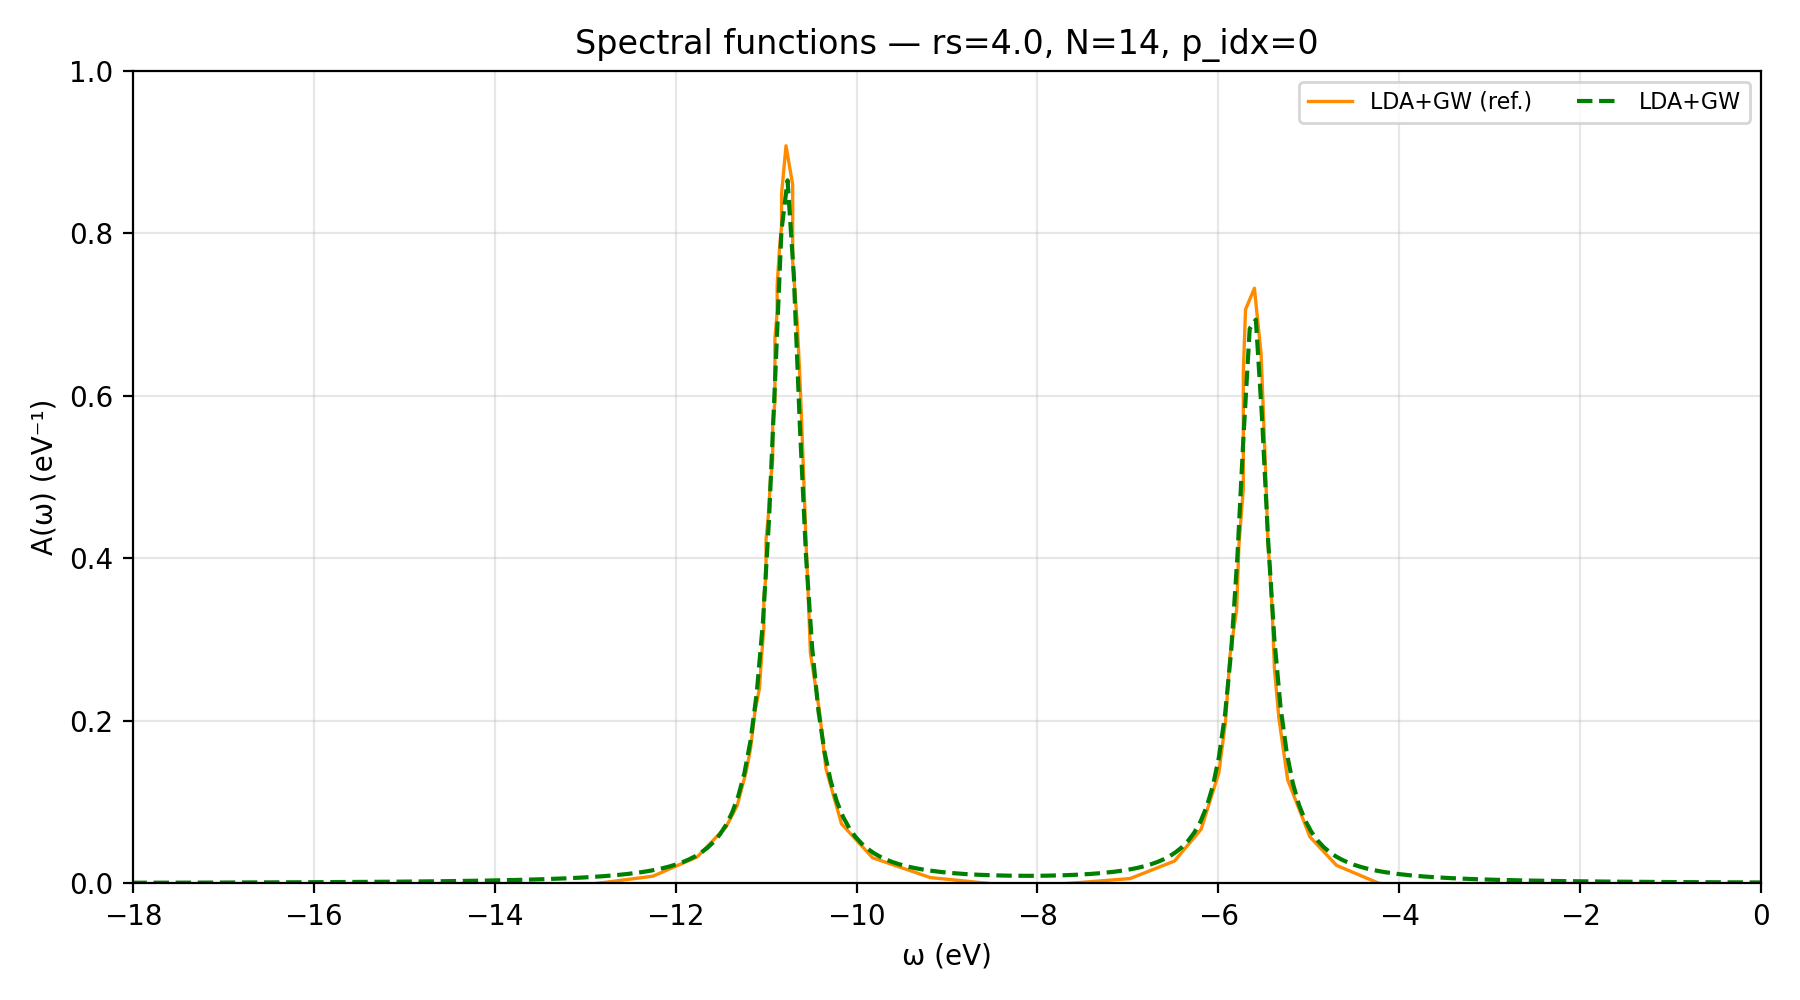
\includegraphics[width=\textwidth]{figs/5-29/mC.png}
        % \caption{LDA+GW}
    \end{figure}
\end{frame}
\begin{frame}
    \frametitle{LDA+GW+C}
    \begin{figure}
        \centering
        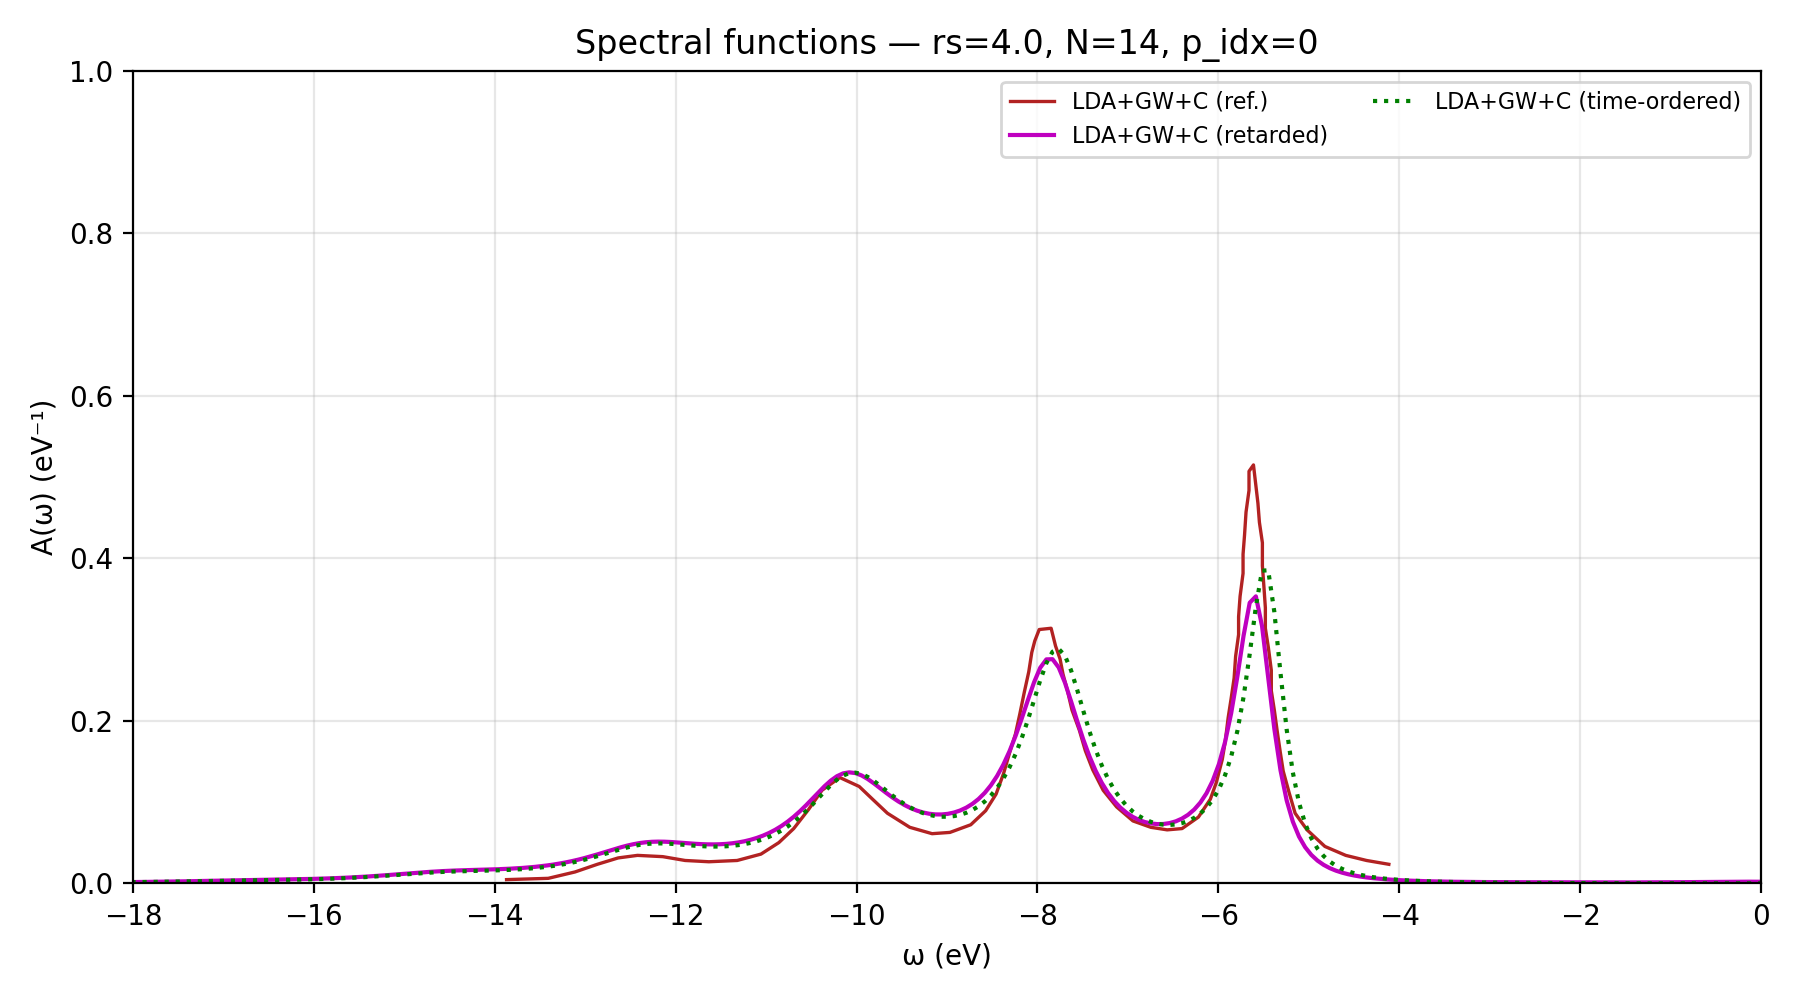
\includegraphics[width=\textwidth]{figs/5-29/pC.png}
        % \caption{LDA+GW}
    \end{figure}
\end{frame}
\begin{frame}
    \frametitle{Green's function}
    \begin{figure}
        \centering
        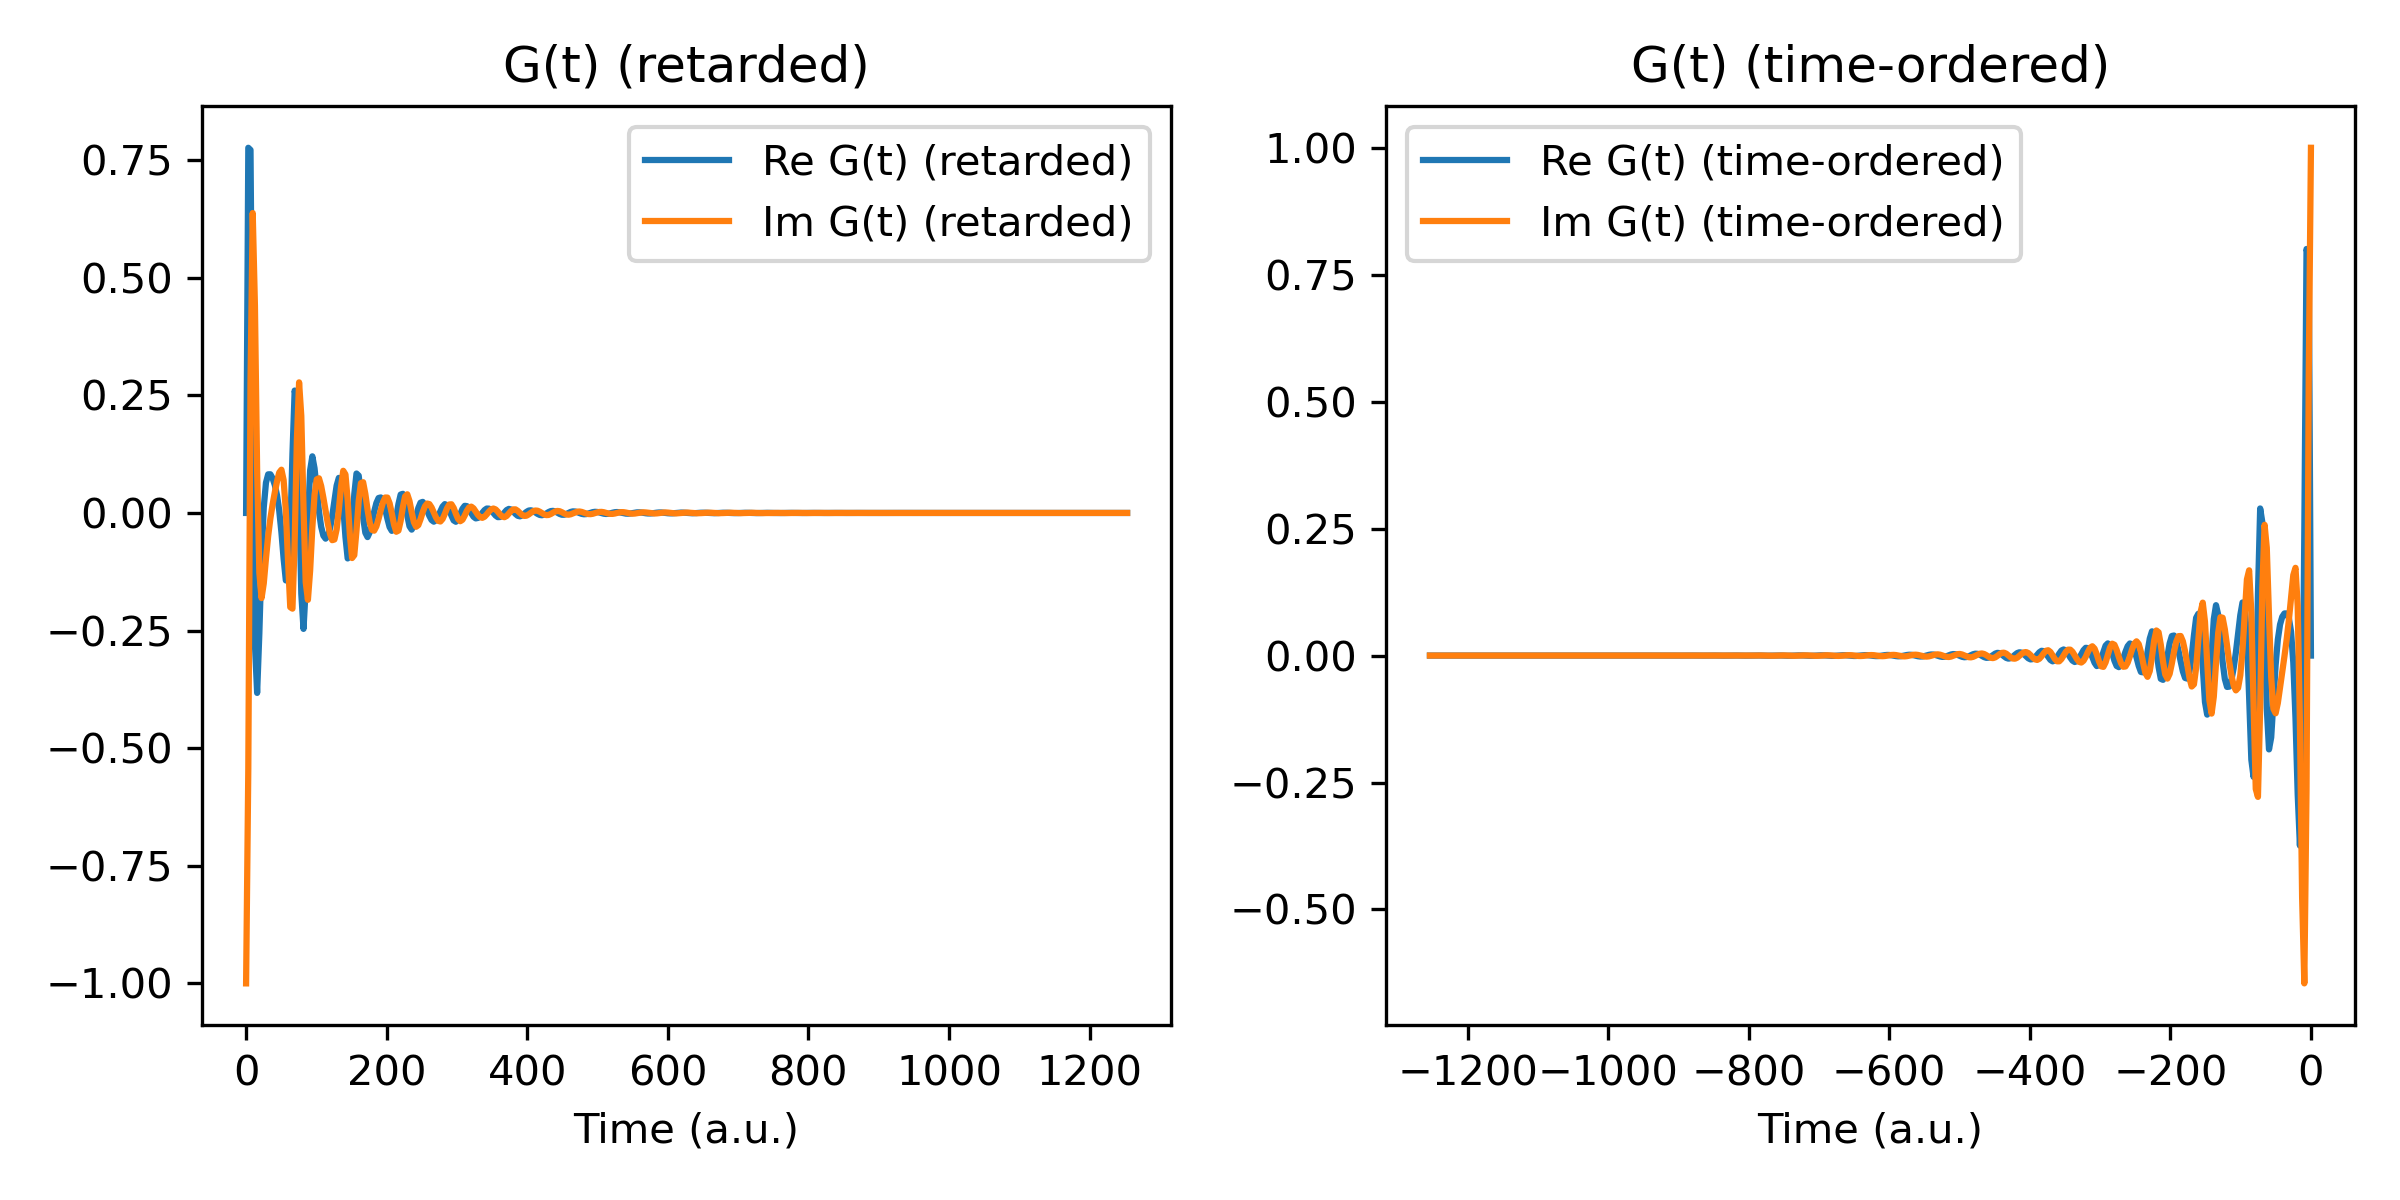
\includegraphics[width=\textwidth]{figs/5-29/gt1.png}
        % \caption{LDA+GW}
    \end{figure}
\end{frame}
\begin{frame}
    \frametitle{Cumulant}
    \begin{figure}
        \centering
        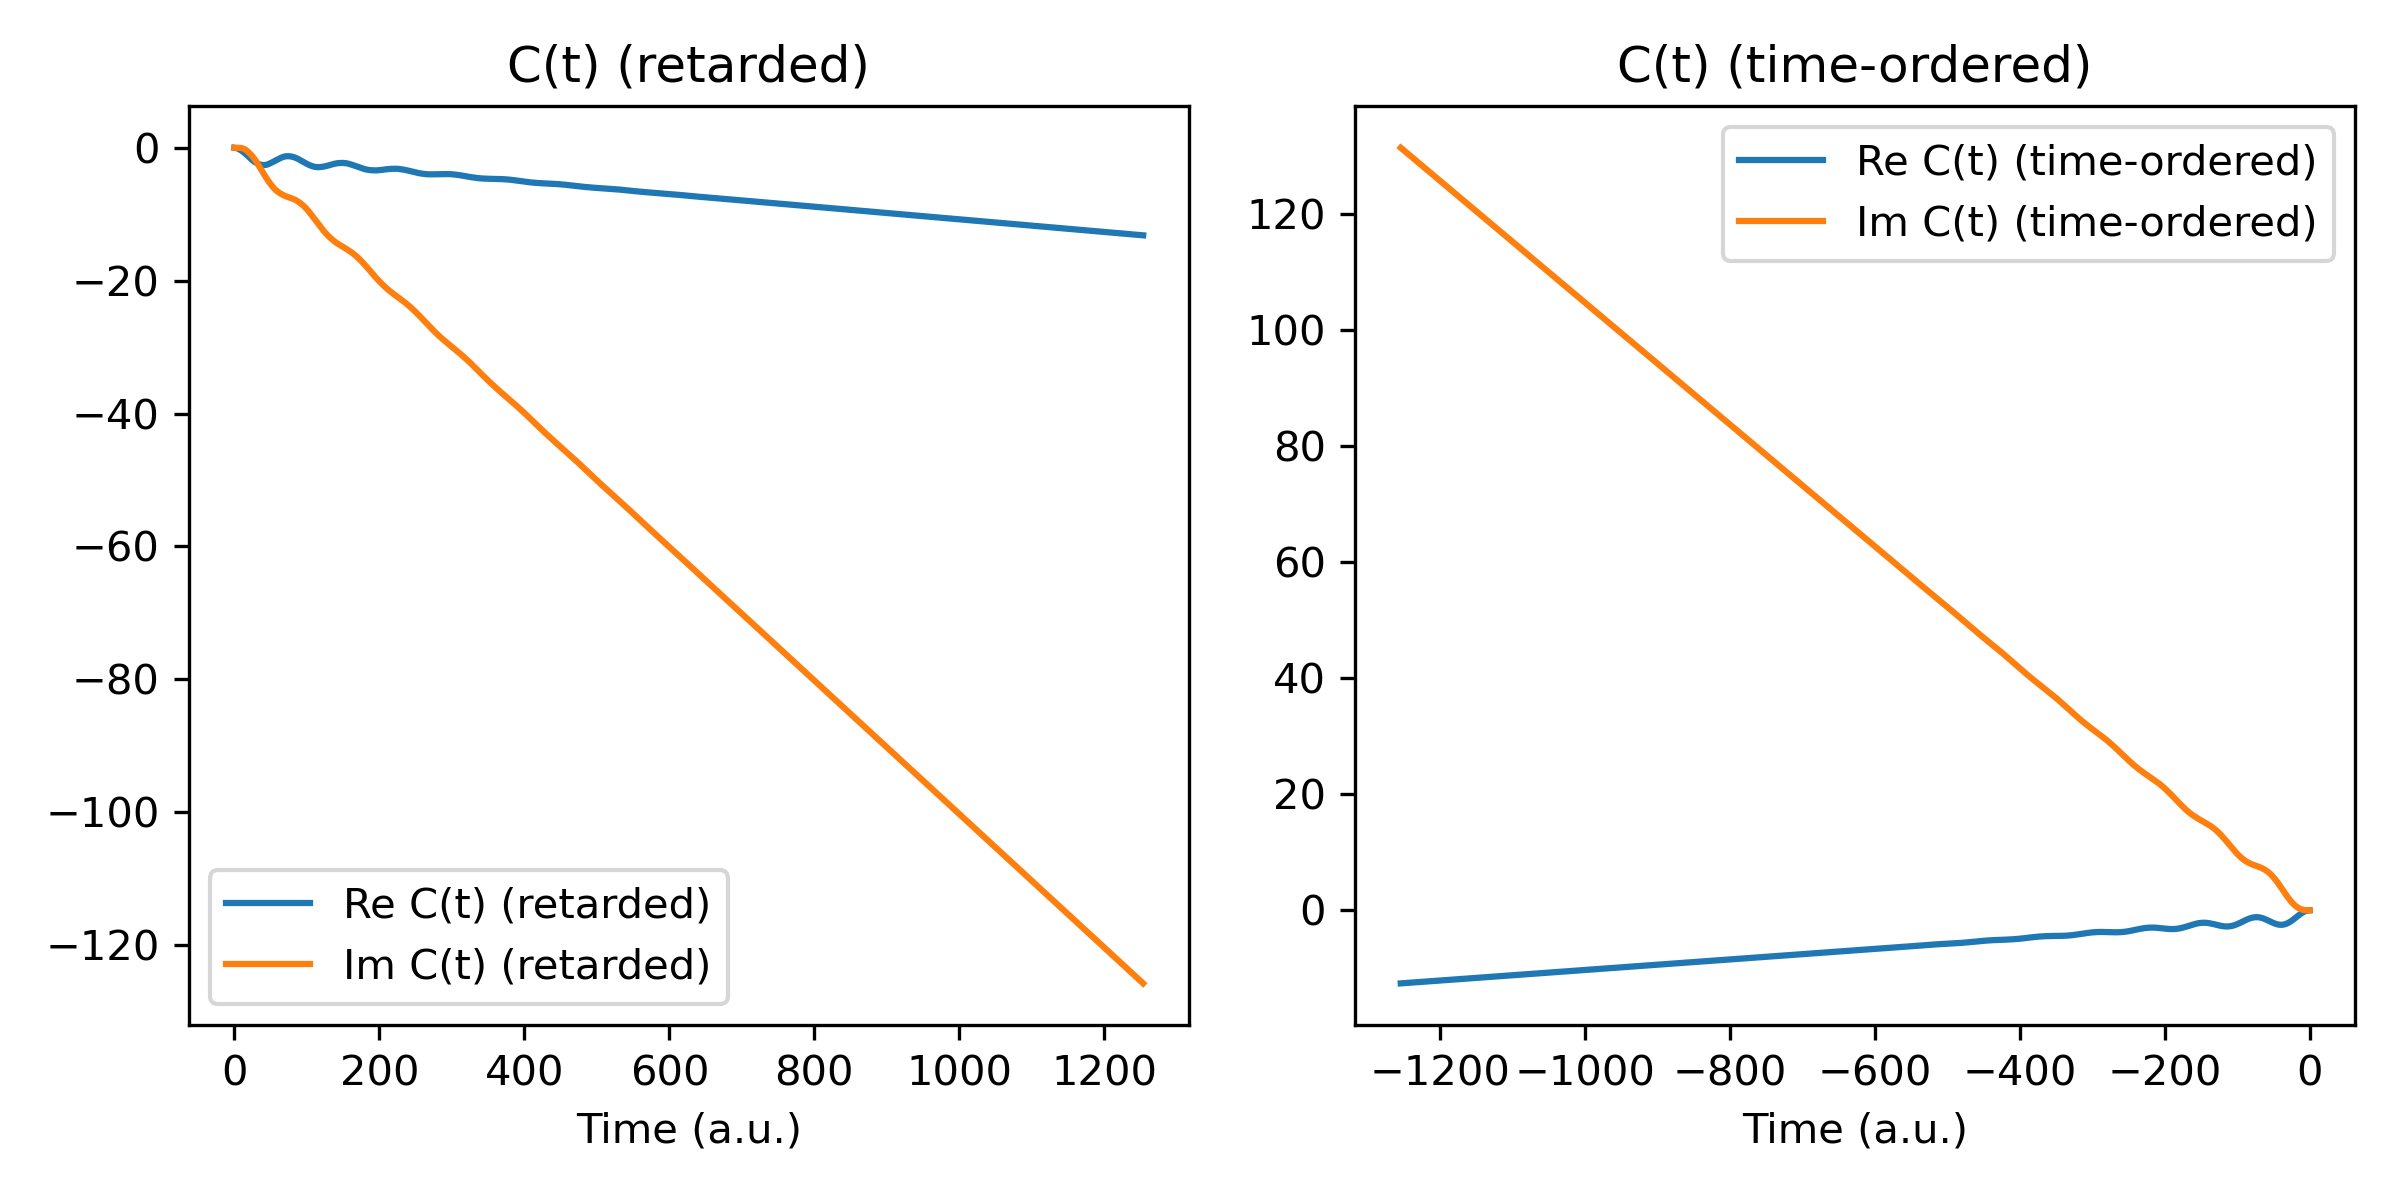
\includegraphics[width=\textwidth]{figs/5-29/ct.png}
        % \caption{LDA+GW}
    \end{figure}
\end{frame}
\section{What to try next}
\begin{frame}
    \frametitle{What to try next}
\begin{itemize}
\item Matching LDA+GW to PySCF\pause
    \item Finite size corrections to the correlation self energy\pause
    \item A self consistent GW reference
\end{itemize}
\end{frame}
